% [page size, font size, recto-verso]{style of the document}
\documentclass[a4paper, 12pt, oneside]{report}

% Encoding of this file. On Linux, all files are UTF8 encoded.
\usepackage[utf8x]{inputenc}

% To write mathematical formula:
% \begin{align} ... \end{align}, \begin{equation} ... \end{equation}
\usepackage{amsmath, amssymb}

% To insert graphics:
% \includegraphics[options]{path}
\usepackage{graphicx}

% The allowed type of image files.
\DeclareGraphicsExtensions{.pdf, .png}

% To include code file without any layout
% \verbatiminput{path}
\usepackage{verbatim}

% To include PDF files
% \includepdf[pages = z,x-y]{path}
\usepackage{pdfpages}

% To do tables on many pages
% \begin{longtable}{define the columns} ... \end{longtable}
\usepackage{longtable}


\textwidth=16cm
\oddsidemargin=0pt
\evensidemargin=0pt

%% The 3 variables which you must initialize:
% Title of the document,
\newcommand{\titleVariable}{Obstacledetector}
% The author(s),
\newcommand{\authorVariable}{Rik Smit}
% The date of the first release.
\newcommand{\firstRelease}{}

\usepackage{hyperref}
% To create all hypertext links for the bibliography, the figures, the bookmarks etc.
% \url{http://www.thewebsite.org}
\hypersetup{
%   backref=true,
%   pagebackref=true,
%   hyperindex=true,
    colorlinks=true,
    breaklinks=true,
    urlcolor= blue,
    linkcolor= blue,
%   bookmarks=true,
    bookmarksopen=true,
    pdftitle={\titleVariable},
    pdfauthor={\authorVariable},
    pdfsubject={Documentation}
}

\title{\titleVariable}
\author{\authorVariable}


\date{\centering First release: \firstRelease \\ Last modification: \today}

\begin{document}
\maketitle

\chapter{The Obstacledetector}

This document explains how to use the $obstacledetector$ module. 
Also see the document ``Obstacle Avoidance'' on how to use it in the architecture.

The obstacle detection module ``obstacledetector.py'' is located in the ``brain/src/vision/'' folder. 
For the detection it uses some modules located in the ``brain/src/vision/obstacledetectorutil/'' folder. 
The obstacle detector will run as a vision module and puts the obstacle matrix in memory.

\begin{figure}[H]
    \centering
    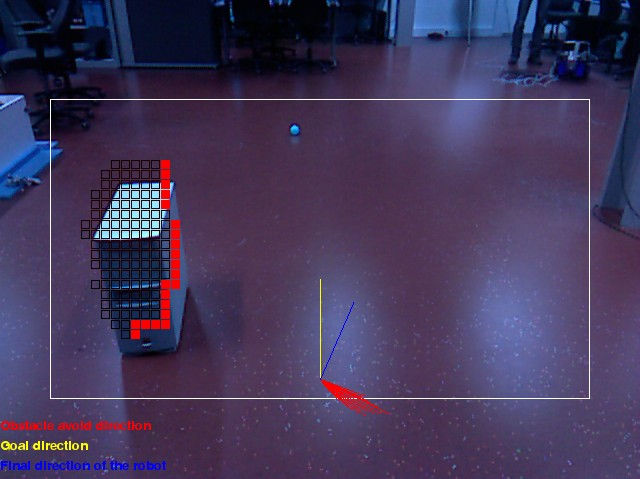
\includegraphics[width=0.9\textwidth]{img/obstacledetector_example.png}
    \caption{Screenshot of the obstacledetector module.\label{fig:example}}
\end{figure}

\section{The Obstacle Matrix}

The obstacle detector converts Kinect depth images to obstacle matrices. 
The size of the obstacle matrix depends on the size of the region of interest (white rectangle in picture above, see below for info) and the size of each segment in that region (size of each square in picture above). 
Currently the matrix size is about 50x20. 
Each element in the matrix contains a single value. 
The value is 0 if no obstacle is detected at that point in the image. 
The value is greather than 0 if there is an obstacle detected at that point in the image. 
In the picture above every visible square represents an item in the matrix with a value > 0. 
In general, the higher the value, the closer the obstacle with respect to the floor. Items with the value 0 are not shown.

\section{Adjusting the Detector}

The region of interest (see below) of the obstacle detector can be adjusted. 
The dimensions can be specified in ``segmentizer.py'' (in vision/obstacledetectorutil/).

Here, also the size of the segments used for detection can be adjusted. 
Current default is 10px by 10px. 10 by 10 is a nice value for detection. 
Making the segment smaller will increase precision, but also the computational power needed. 
It's not recommended making the segment size larger as it might overlook obstacles during detection.

When the spotted distance to a segment in the region is smaller then the (calibrated) distance to the floor in the same segment, the obstacle detector knows there is an obstacle there. 
The threshold is specified in the variable 'distanceDifference' in the function 'getObstacleMatrix()' in the obstacle detector. 
Currently it is set to 2, which is a safe value. 
Making it smaller will allow the obstacle detector to spot smaller obstacles. 
It will also increase the chance to see the entire floor as an obstacle. 
This will happen faster when the Kinect is waggling a lot. 
Enlarge the value if the floor is very bumpy (like outside). 
With the current value it will NOT spot the doorstep.

\section{Calibration}

Before using the obstacle detector you want to calibrate it. 
The calibration procedure will calculate the distances to the floor and save them to a calibration file located in ``vision/obstacledetectorutil/''. 
The file is called ``calibration.data''. 
Every time the orientation of the Kinect is changed you want to recalibrate. 
Every time you change the detection region (see above), you need to recalibrate. 
Every time you change the segment size (number of pixels used for a segment in the region), you need to recalibrate. 
Calibration is done by the calibrator in ``brain/src/vision/obstacledetectorutil/calibrator.py''. 

Before calibrating make sure the Kinect looks at a clear floor so no objects are in the region of interest.
Do ``python calibrator.py kinect 50'' to calibrate.
This will calibrate the obstacle detector using 50 images from the Kinect. 
These are also the defaults. 
While calibration (takes about 3 seconds) you might want to waggle the top of the robot a bit to simulate its movement as if the robot was driving. 
This will increase the robustness of the obstacle detector.

\section{Region of Interest}

Kinect images are 640px by 480px. 
Only a specific region of this image is used for detection (white rectangle in the picture above). 
This region can be specified when instantiating an ObstacleDetector() object. 
The default region is specified in the ``obstacledetector.py'' file. 
It is specified by an tuple (left, top, width, height). 
Don't mess around with the values too much. 
Right now it uses a decent region of the image so not a to large clear floor area is needed for calibration. 
You might want to adjust the 'top' parameter when the front of the robot is visible in the region. 
You don't want the front of the robot to be visible in the region.

\end{document}
